\documentclass[12pt,a4paper,utf8x]{report}
\usepackage [english]{babel}

% Pour pouvoir utiliser 
\usepackage{ucs}
\usepackage[utf8x]{inputenc}

\usepackage{url} % Pour avoir de belles url
\usepackage {geometry}

% Pour mettre du code source
\usepackage {listings}
% Pour pouvoir passer en paysage
\usepackage{lscape}

% Pour pouvoir faire plusieurs colonnes
\usepackage {multicol}
% Pour crééer un index
\usepackage{makeidx}
\makeindex

% Pour gérer les liens interractifs et les signets Acrobat
\usepackage{hyperref}
\hypersetup{
pdftitle={titre de mon document},
pdfauthor={DEJEAN Charles, POTTIER Vincent},
pdfsubject={Sujet du document},
pdfkeywords={les mots clefs},
bookmarks, % Création du signet
pdfstartview=FitH, % Page de la largeur de la fenêtre
colorlinks=true, % Liens en couleur
linkcolor=black, 	
anchorcolor=black, 	
citecolor=black, 	
filecolor=black, 	
menucolor=black,
runcolor=black,
urlcolor=black, 	
frenchlinks=black,
bookmarksnumbered=true, % Signet numéroté
pdfpagemode=UseOutlines, % Montre les bookmarks.
bookmarksopen =true,
}

% Pour afficher la bibliographie, mais pas nottoc (Table of Contents), notlof (List of Figures) ni notlot (List of Tables)
\usepackage[notlof, notlot]{tocbibind}


% Pour les entetes de page
% \usepackage{fancyheadings}
%\pagestyle{fancy}
%\renewcommand{\sectionmark}[1]{\markboth{#1}{}} 
%\renewcommand{\subsectionmark}[1]{\markright{#1}} 

% Pour l'interligne de 1.5
\usepackage {setspace}
% Pour les marges de la page
\geometry{a4paper, top=2.5cm, bottom=3.5cm, left=1.5cm, right=1.5cm, marginparwidth=1.2cm}

\parskip=5pt %% distance entre § (paragraphe)
\sloppy %% respecter toujours la marge de droite 

% Pour les pénalités :
\interfootnotelinepenalty=150 %note de bas de page
\widowpenalty=150 %% veuves et orphelines
\clubpenalty=150 

%Pour la longueur de l'indentation des paragraphes
\setlength{\parindent}{15mm}

%%%% debut macro pour enlever le nom chapitre %%%%
\makeatletter
\def\@makechapterhead#1{%
  \vspace*{50\p@}%
  {\parindent \z@ \raggedright \normalfont
    \interlinepenalty\@M
    \ifnum \c@secnumdepth >\m@ne
        \Huge\bfseries \thechapter\quad
    \fi
    \Huge \bfseries #1\par\nobreak
    \vskip 40\p@
  }}

\def\@makeschapterhead#1{%
  \vspace*{50\p@}%
  {\parindent \z@ \raggedright
    \normalfont
    \interlinepenalty\@M
    \Huge \bfseries  #1\par\nobreak
    \vskip 40\p@
  }}
\makeatother
%%%% fin macro %%%%

%Couverture 
\title
{
	\normalsize{Master ALMA Nantes\\
	Université de Nantes\\
	2009-2010}\\
	\vspace{15mm}
	\Huge{Project Report for Technique de Développement}
}
\author{DEJEAN Charles, POTTIER Vincent\\
	\vspace{45mm}
}



\begin{document}

\maketitle

%Remerciements

Je tiens à remercier :
et on met la liste des personnes que l'on remercie. Toto, tutu, titi. et on met la liste des personnes que l'on remercie. Toto, tutu, titi.et on met la liste des personnes que l'on remercie. Toto, tutu, titi.et on met la liste des personnes que l'on remercie. Toto, tutu, titi.


Et on met la liste des personnes que l'on remercie. Toto, tutu, titi.et on met la liste des personnes que l'on remercie. Toto, tutu, titi.et on met la liste des personnes que l'on remercie. Toto, tutu, titi.et on met la liste des personnes que l'on remercie. Toto, tutu, titi.et on met la liste des personnes que l'on remercie. Toto, tutu, titi.

%\clearpage

\tableofcontents
\clearpage

% Pour avoir un interligne de 1,5
\begin{onehalfspace}

\chapter{Implemetation}

	Here are the UML diagrams which discribe our data structure, artificial intelligence and user interface.

	\section{Game data structure}

	\begin{figure}[!]
  		\begin{center}
		\scalebox{0.7}{
  		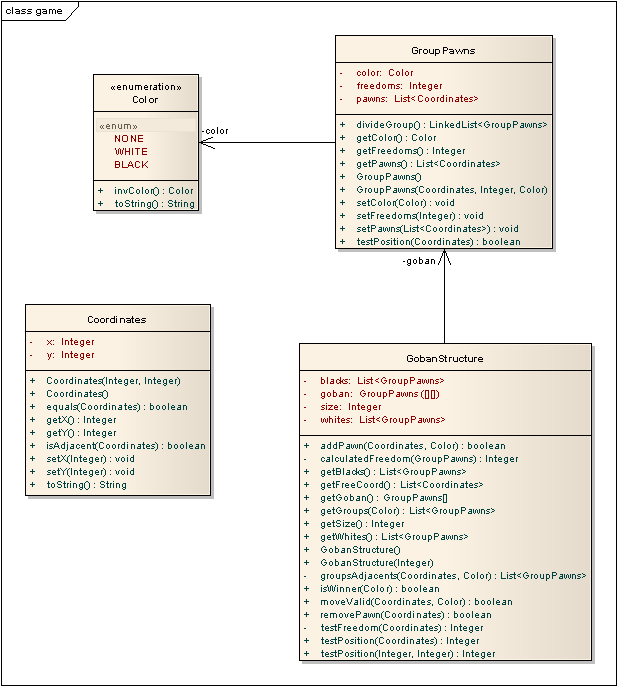
\includegraphics{game}
		}
  		\end{center}
		\caption{Game date structure UML Diagram}
	\end{figure}

	\subsection{Coordinates}
			
		A simple data storage class which allow to store coordinates (two number) and to compare two coordinates.

	\subsection{Color}
		
		A simple class which allow to easily identify the color of a piece or a group of piece.
		
	\subsection{GroupPawn}
		
		This class allow to manage a group of piece. It is composed of a list of coordinates, its color and its number of freedom.
		Methods update the contents of the group, when a piece is added or removed.
		
	\subsection{GobanStructure}

		This is the main class of the game : every action done during the game pass through this class. It contains two lists of all groups (one by color), the goban size (9 by default) and the game grid (a 2 dimensions array), where every case contains a reference to a group of pieces which contains the piece itself.
		
	\section{Artificial Intelligence}

	\begin{figure}[!]
  		\begin{center}
		\scalebox{0.7}{
  		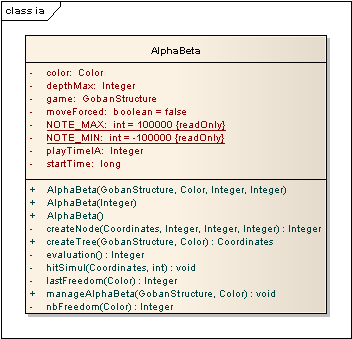
\includegraphics{artInt}
		}
  		\end{center}
  		\caption{Artificial Intelligence UML Diagram}
	\end{figure}

	The artificial intelligence is based on the Alpha-beta algorithm, which has been learned during AI lessons. The hardest part of this algorithm is the evaluation function, which note a goban plate state. A good note implies a good situation for a color, and a bad note, a bad situation.

	Considering this function, we had focus on !
\begin{itemize}
\item A win move : We have tried to make that our AI select a win move. It looks easy, but in fact, the Alpha-Beta can let go a win move ...
\item A loose move : We have forced the AI to play in order to save its life, as a top priority.
\item Decrease the freedom of the opponent : In order to have an aggressive AI, we forced it to decrease the freedom of the opponent. It simulates more a living partner than a stupid AI.
\end{itemize}
	
	\section{User Interface}

	\begin{figure}[!]
  		\begin{center}
		\scalebox{0.7}{
  		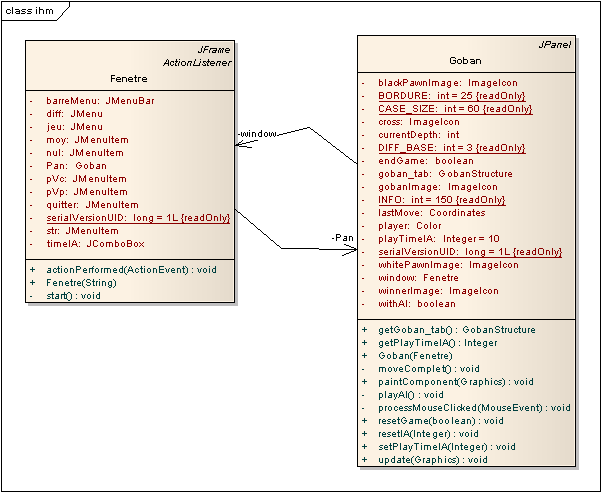
\includegraphics{ihm}
		}
  		\end{center}
  		\caption{User Interface UML Diagram}
	\end{figure}

		We used the usual fonctionnality offerd by Java Environment (swing and awt), which allows us to create a sober user interface.

	
\clearpage


\chapter{User Manual}

\section{User Interface}

	\subsection{Game Launch}
		When you launch the game, a match versus an Artificial Intelligence begin. The player (you) begins always et play with black stones.
		
	\subsection{Kind of games}

		The User Interface allows to modify the AI difficulty or the kind of game ( Player vs Player or Player vs AI), with the selection tab at the tab of the window.

		It is possible to configure the maximum thinking's time of the AI by the menu at the bottom right of the window.
	
	\subsection{End of game}
		When a player captures at least one opponent's stone, he wins. A simple clic starts another match from the same kind of the previous.
		
\section{Game install}
	
	There is nothing to really install. In order to play, you juste have to run the mainIhm class, in the main package.
	
	
\clearpage




% Pour finir l'interligne de 1,5
\end{onehalfspace}

%----------------------------------------
% Pour la bibliographie
%----------------------------------------
% Citer tous les ouvrages/références
%\nocite{*}
% Trier par ordre d'apparition
%\bibliographystyle{unsrt}
% Pour le style de la biblio
%\bibliographystyle{plain.bst}
% Ecrire la biblio ici
%\bibliography{biblio}

\printindex

\appendix


\end{document}
